\documentclass[12pt,a4paper]{book}  % -*- mode: latex; mode: auto-fill -*-

%pdftex stuff ...
\newif\ifpdf
\ifx\pdfoutput\undefined
  \pdffalse
\else
  \pdfoutput=1
  \pdftrue
\fi

\ifpdf
  \usepackage[pdftex]{graphicx}
  \pdfcompresslevel=9
\else
  \usepackage{graphicx}
\fi

\usepackage{fancyhdr}
\usepackage{listings}

\lstdefinelanguage{Gap}%
  {keywords={while,for,in,do,od,repeat,until,if,then,else,elif,fi,
      function,end,local,return,true,false,rec,quit,break,not,gap},%
  sensitive=true,%
  commentline={\#},%
  blankstring=true,%
  indent=2em,%
%  frame=tlbr,%
  stringizer=[b]{"'}%
}%
\lstset{language=Gap,basicstyle=\small}

\newcommand{\GAP}{\textsf{GAP}}
\newcommand{\gap}{\textsf{GAP}}
\newcommand{\XGAP}{\textsf{XGAP}}
\newcommand{\GASP}{GASP}
\newcommand{\gasp}{GASP}
\newcommand{\abstractname}{Abstract}
\newenvironment{abstract}{\section{Abstract}}{}
\def\abstract{\section*{\centering\abstractname}}
\def\endabstract{\medbreak}
\newenvironment{acknowledgements}%
   {\renewcommand{\abstractname}{Acknowledgements}%
    \begin{abstract}}
   {\end{abstract}}

\title{
   GASP: A Computing Framework For Markov Chain Monte Carlo Spatial Problems
   \footnote{Submitted in partial fulfilment 
   of the requirements for the Bachelor 
   of Science degree with Honours at the 
   University of Western Australia}
}
\date{October 2000}
\author{James Henstridge}

\begin{document}

\ifpdf
  \DeclareGraphicsExtensions{.png,.pdf}
\else
  \DeclareGraphicsExtensions{.eps}
\fi

\maketitle

\begin{abstract}
In the area of Markov Chain Monte Carlo spatial problems, not many
general purpose simulation systems exist.  The GASP package is a
framework for writing simulations.  GASP stands for
\emph{\textbf{G}enerating \textbf{A}lgorithms for \textbf{S}patial
\textbf{P}atterns}.  It is designed to handle as many
different problems as possible.  A number of algorithms are
distributed with the GASP framework, including a simulation of the
Strauss Process using the Metropolis-Hastings Algorithm.

GASP includes a graphical user interface that aids visualisation of an
algorithm, and sophisticated logging capabilities which allow for
detailed post-simulation analysis.  It is implemented as a share
package for the computer algebra system \GAP.
\end{abstract}

\begin{acknowledgements}
\noindent Thank you to my supervisors Adrian Baddeley and Alice
Niemeyer.

\noindent Thank you to Alexander Hulpke for information about \GAP.

\noindent Thank you to Ute Hahn for background information on some of the
algorithms I considered.
\end{acknowledgements}


\tableofcontents

% -*- mode: latex; mode: auto-fill -*-

\chapter{Introduction}

\section{Aims}

In this project, I looked at the problem of implementing a framework
for simulating processes related to spatial statistics using
algorithms such as the Metropolis-Hastings algorithm.

The aim of the project was to produce a framework that could handle as
many different algorithms in the class as possible, while remaining
simple enough to be understood and easy to use.  The result is the
GASP package \cite{gasp-source}, which stands for
\emph{\textbf{G}enerating \textbf{A}lgorithms for \textbf{S}patial
\textbf{P}atterns}.

\section{The Choice of Language}

Simulations of this type often require a lot of computation, so have
traditionally been implemented in languages such as C or C++, due to
the speed and flexibility they give.  Using such a language has
drawbacks:

\begin{itemize}
\item a program would be written specifically for a particular
problem, so may require substantial modification to cover a different
problem.
\item knowledge of the C language, which includes many details, such
as memory management, that are not directly related to the problem.
This significantly raises the barrier for someone wanting to use such
a program.  Also, C is perceived as being difficult to learn, which
reduces the value of a system which is aimed at mathematicians.
\item as C is a compiled language, it takes more effort to make a
change to the algorithm, which can slow down development.
\end{itemize}

Rather than having many programs, each implementing their own
algorithm, it would be better to have a framework from which many
different algorithms could be explored with.  That was the aim of
my project.

An interpreted language was chosen because of reduced development
overhead, allowing more rapid experimentation and implementation of
new algorithms.

\section{\GAP}

The language chosen for the implementation was \GAP{} \cite{gap-www}.
While \GAP{} was originally designed for work with group theory, a
number of its features made it an interesting choice for this class of
problem.

While S-Plus \cite{s-plus} may be considered the obvious choice of
language, it suffers from some problems when used to run simulations
that take a long time.  Problems related to instability and memory
leaks are magnified during long runs, which may lead to loss of data
if the interpreter crashes.  Also, to someone who does not already
know S-Plus, the syntax can be difficult to learn.

Like S-Plus, \GAP{} is an interpreted language.  Its syntax was
designed with mathematicians in mind, so is quite easy for a new user
to pick up.  \GAP{} has some object oriented features, which were used
when implementing the GASP framework.

As well as having the rapid development advantages of interpreted
languages, \GAP{} also has interactive debugging features, and support
for designing graphical user interfaces that consist of menus and
geometric shapes drawn on a canvas.

Using \GAP{}'s ability to pass functions as arguments to other
functions, GASP allows the user to hook into many different parts of
the simulation framework.

\section{The Change Log}

All the algorithms that I considered involved transitions between
different states of a configuration of some type of object such as
points in the plane.  Quite often, it is these transitions, or changes
in the configuration, that are interesting.

In the GASP framework, these changes form an important part of the
simulation.  Borrowing some ideas from the undo capabilities found in
some software, all changes made to the configuration are encapsulated
inside objects that hold all information to apply and revert the
change in state.

As the amount of memory required to encode these these changes is
generally smaller than the amount required for the configuration
itself, it was feasible to log a lot more information about what
happened during the simulation than with systems where the complete
state of the configuration was logged.  This unique feature of GASP
gives users the ability to analyse a simulation much more effectively,
even after the simulation has completed.

\section{Chapter Guide}

The second chapter gives a brief overview of the mathematics behind
some of the problems that the GASP framework covers.

The third chapter covers the features of \GAP{} that were useful when
designing GASP, and more detailed reasons why it was chosen as the
language to implement GASP in.

The fourth chapter is an introduction to the functionality provided by
the GASP framework.  This chapter is aimed at users who are interested
in using the existing functionality in GASP, rather than extending it
to handle new algorithms.

The fifth chapter looks at the implementation of the framework, and
how to extend its functionality -- both the algorithms that are
supported and the types of configurations that can be used in
simulations.


% -*- mode: latex; mode: auto-fill -*-
\chapter{Background of Class of Problems}

\newtheorem{algorithm}{Algorithm}

Some knowledge of the underlying probability theory is required to
fully understand the purpose and functionality of the software we
developed.  So we will first look at some of the basic concepts and a
few problems that relate to the program.  Some of the background
material in this chapter can be found in \emph{Spatial Statistics}
\cite{spatial-stats}.

\section{Markov Chains}

\subsection{Basics}

A Markov Chain is a system with a number of possible states, and
probabilistic rules for moving between those states.  As we move
through time, we make transitions between states.  There are rules
that govern to which state we can move from the current one.  The
restriction on the rules is that given the entire past series of
states $X_1, X_2, \ldots, X_t$, the choice of next state $X_{t+1}$
only depends on the current state $X_t$.

We can represent the probabilities for moving from a given state $X_t$
to each of the other states in the system by the vector $P_t =
(p_{t1}, p_{t2}, \ldots, p_{tn})$, where $p_{ti}$ is the probability
of moving from state $X_t$ to state $X_i$.  We can collect the
probability vectors for transitions from each state into a matrix:
\begin{equation}
\mathbf{P} = \left(\begin{array}{c}
P_1 \\
P_2 \\
\vdots \\
P_n
\end{array}\right)
\end{equation}


\noindent This matrix, known as the \emph{transition probability
matrix}, is \emph{stochastic}.  That is the sum of the entries in each
row is one (as the rows represent the complete set of probabilities
for moving to any state in the state space).

If the current state is randomly distributed in the state space
according to the probability row vector $\pi_t$, we can get the
distribution for the next state by right multiplication by
$\mathbf{P}$:
\begin{equation}
\pi_{t+1} = \pi_t \mathbf{P}
\end{equation}

\noindent Similarly, we can get the distribution for the state after that
by multiplying the probability distribution vector by $\mathbf{P}$ again.

Some systems will converge towards an \emph{limiting} distribution as
they progress in time.  This distribution is often denoted $\pi$.  The
limiting distribution's definition is as expected:
\begin{equation}
\pi = \lim_{i \to \infty}\pi_0 \mathbf{P}^i
\end{equation}


%XXXX
\noindent If such a limit exists, then under certain circumstances
$\pi$ is an equilibrium distribution, in which case it satisfies
\begin{equation}
\pi = \pi \mathbf{P}
\end{equation}


\noindent This corresponds to the simple linear system $\pi(\mathbf{P}
- \mathbf{I}) = 0$, which can be solved to find the possible
equilibrium distributions for the system.

\subsection{The Monte Carlo Method}

The \emph{Monte Carlo} method is a method of solving problems using
random numbers.  We can apply these ideas when simulating a Markov
Chain system \cite{mcmc-in-practice}.

If we know the state transition probability matrix $\mathbf{P}$ for a
system, it is possible to simulate a Markov Chain.  The algorithm
proceeds as follows:

\begin{algorithm}[Monte Carlo]
\ 

\begin{enumerate}
\item Pick an initial state $X_0$.

\item Given that the current state $X_t=x$, we generate the next state
$y$ from the random probability distribution $P(X_{t+1}=y) = p_{xy}$,
or the $y$th column of the $x$th row of the transition probability
matrix $\mathbf{P}$.

\item Having picked the new state $X_{t+1}$, we go to step 2 and
repeat to generate the next state.
\end{enumerate}
\end{algorithm}


\subsection{Problems}

Of course, Algorithm 1 is not practicable in all situations.  Some
possible problems are:

\begin{itemize}
\item the state transition matrix $\mathbf{P}$ is not known, or would
be too expensive to calculate.  In this case, we would still need to
know the rule for calculating the next state.
\item the number of possible states in the system is infinite or very
large (for example, the states may represent the positioning of some
points on the plane).
\end{itemize}

In these cases, we might not be able to find the equilibrium
distribution for the system just by solving a system of linear
equations, or may not get a useful result.  However, we may be able to
simulate the system, which is another way to get the desired
information.

\section{Using Simulation to Generate Distributions}

For some probability distributions, it is not clear how to generate
instances of the distribution directly.  Instead, we sometimes use an
iterative Markov Chain based algorithm that will converge to the
desired distribution as equilibrium.

This is similar to shuffling cards in order to randomise their order.
We know the distribution that we want -- we just need to find a
`shuffling' algorithm that will get us to that distribution.  One such
algorithm is the Metropolis-Hastings Algorithm.

\subsection{Metropolis-Hastings Algorithm}

The \emph{Metropolis-Hastings} algorithm is a Markov Chain system that
can be used to generate a realisation of a given equilibrium
distribution.

It uses the idea that if the probability of the transition from state
$x$ to state $y$, is the same as for the transition $y \to x$, then
the equilibrium distribution will be maintained.  This is known as
\emph{detailed balance}, as expressed in Equation
\ref{eq:detailed-balance}.
\begin{equation}\label{eq:detailed-balance}
\mathbf{P}(X_t = x\ \mathbf{and}\ X_{t+1} = y) =
   \mathbf{P}(X_t = y\ \mathbf{and}\ X_{t+1} = x)
\end{equation}


\noindent It is achieved using the algorithm described below.  It
consists of a proposal step and an acceptance step.

\begin{algorithm}[Metropolis-Hastings]
\ 

\begin{enumerate}
\item An initial state $x$ is chosen.
\item proposal: a transition $x \to y$ is proposed.  The transition is
chosen randomly according to some predefined random method with
probability $p_{prop}(x \to y)$.
\item acceptance check: the probability of accepting this transition
$p_{acc}(x \to y)$ is calculated.  With probability $p_{acc}(x \to
y)$, we move to state $y$.  Otherwise we stay at $x$.
\item go to step 2 and repeat.
\end{enumerate}

According to these rules, the probability that the next state
($x_{i+1}$) will be $y$, given the current state ($x_i$) is $x$, is:
\begin{equation}\label{eq:p-trans-def}
p_{trans}(x \to y) = p_{prop}(x \to y) p_{acc}(x \to y)
\end{equation}
\end{algorithm}

\noindent Applying the fact that $\mathbf{P}(A\ \mathbf{and}\ B) =
\mathbf{P}(A\ |\ B) \mathbf{P}(B)$ to both sides of Equation
\ref{eq:detailed-balance} and substituting $p_{trans}(x \to y)$ we
get:
\begin{equation}
p_{trans}(x \to y) \mathbf{P}(X_t = x) =
   p_{trans}(y \to x) \mathbf{P}(X_t = y)
\end{equation}

\noindent Substituting from Equation \ref{eq:p-trans-def}:
\begin{equation}
p_{acc}(x \to y) p_{prop}(x \to y) \mathbf{P}(X_t = x) =
   p_{acc}(y \to x) p_{prop}(y \to x) \mathbf{P}(X_t = y)
\end{equation}

\noindent And rearranging, we get:
\begin{equation}
\frac{p_{acc}(x \to y)}{p_{acc}(y \to x)} =
  \frac{p_{prop}(y \to x) \mathbf{P}(X_t = y)}{
        p_{prop}(x \to y) \mathbf{P}(X_t = x)}
\end{equation}

\noindent We need to choose values $p_{acc}(x \to y)$ and $p_{acc}(y
\to x)$ that will satisfy equation.  The ratio $\frac{p_{acc}(x \to
y)}{p_{acc}(y \to x)}$ is known as \emph{Green's Ratio}, or $R_{x \to
y}$.  The probabilities $\mathbf{P}(X_i = y)$ and $\mathbf{P}(X_i =
x)$ are given in the desired equilibrium distribution.  The proposal
probabilities $p_{prop}(x \to y)$ and $p_{prop}(y \to x)$ were chosen
as part of the algorithm.  Hence, we can calculate $R_{x \to y}$.

For the Metropolis-Hastings algorithm, we set $p_{acc}(x \to y)$ as:

\begin{equation}
p_{acc}(x \to y) = \min(\{R_{x \to y}, 1\})
\end{equation}


\noindent In the case that $R_{x \to y} > 1$, $R_{y \to x} = 1 / R_{x
\to y} < 1$, so $\frac{p_{acc}(x \to y)}{p_{acc}(y \to x)} =
\frac{1}{1 / R_{x \to y}} = R_{x \to y}$.  When $R_{x \to y} < 1$, we
get $\frac{p_{acc}(x \to y)}{p_{acc}(y \to x)} = \frac{R_{x \to y}}{1}
= R_{x \to y}$.  So this definition of $p_{acc}(x \to y)$ is
consistent.  For a system with an infinite number of states, we can
use the corresponding probability densities in place of the discrete
measures, and the same argument applies.

Of course, the Metropolis-Hastings Algorithm does not guarantee that
we will converge on the desired equilibrium distribution.  Even in the
case where it does converge, it does not give any indication when we
have converged to the desired equilibrium distribution.


\subsection{The Metropolis-Hastings Algorithm and Point Processes}
\label{sect:mh-points}

Point processes are spatial models of a collection of points governed
by some probability density \cite{markov-point-processes-2}.  Each
state of the system is a configuration of points within some region
(or window) of the plane.  It can be very difficult to realise the
process directly, so we use an algorithm that will converge to the
desired distribution, such as the Metropolis-Hastings algorithm.

For the proposal part of the algorithm, we will limit the possible
state transitions allowed to (a) adding a new point in a random
location within the window $W$, and (b) removing an existing point.
All other transitions are assigned a probability of zero.  We will
assign equal probability to adding and removing a point (unless the
configuration is empty, in which case only an addition is possible).

We represent the state by the set of points on the plane
$\mathbf{x} = \{ x_1, \ldots, x_n \}$.  The probability density of the
proposal to add a particular point $y$ to the configuration somewhere
in the window of area $|W|$ is $p_{prop}(\mathbf{x} \to \mathbf{x}\cup
\{y\}) = \frac{1}{2} \frac{1}{|W|}$.  Similarly, the probability of
proposing to remove a particular point $y$ is $p_{prop}(\mathbf{x} \to
\mathbf{x}\backslash \{y\}) = \frac{1}{2} \frac{1}{n(\mathbf{x})}$
where $n(\mathbf{x})$ is the number of points in the set $\mathbf{x}$.

Hence, for adding a point, Green's Ratio becomes:
\begin{equation}
  R_{\mathbf{x} \to \mathbf{x} \cup \{y\}} = \frac{|W|}{n(\mathbf{x})
  + 1} \frac{f(\mathbf{x} \cup \{y\})}{f(\mathbf{x})}
\end{equation}

\noindent and for removing a point, we have:
\begin{equation}
  R_{\mathbf{x} \to \mathbf{x} \backslash \{y\}} =
  \frac{n(\mathbf{x})}{|W|} \frac{f(\mathbf{x} \backslash
  \{y\})}{f(\mathbf{x})}
\end{equation}

\noindent where $f(\mathbf{x})$ is the density function for the
equilibrium distribution.

Hence, the acceptance probability $p_{acc}$ used will be $\min(R_{\mathbf{x} \to
\mathbf{x} \cup \{y\}}, 1)$ or $\min(R_{\mathbf{x} \to \mathbf{x}
\backslash \{y\}}, 1)$ respectively.


\section{The Strauss Process}\label{sect:strauss-process}

The \emph{Strauss Process} \cite{strauss-process} is an example of a
point process that can be simulated using the Metropolis-Hastings
algorithm.  The density function for the Strauss Process is:
\begin{equation}\label{eq:strauss-process}
f(\mathbf{x}) = \alpha \beta^{n(\mathbf{x})} \gamma^{s(\mathbf{x})}
\end{equation}

\noindent where $\mathbf{x}$ and $n(\mathbf{x})$ are defined as in
Section \ref{sect:mh-points}, and $s(\mathbf{x})$ is defined as the
number of `close' pairs of points separated by no more than a given
distance $r$.

The symbols in the density function of Equation
\ref{eq:strauss-process} are:
\begin{description}
\item[$\alpha$] is a constant to normalise the function to ensure that it
is a density function.
\item[$\beta$] is a parameter that measures the `intensity' .  It
affects the number of points we would expect to find in the
configuration.
\item[$\gamma$] is the \emph{interaction} parameter:
  \begin{itemize}
  \item If $\gamma = 1$, then the density function does not depend on
  neighbour relationships.
  \item If $0 < \gamma < 1$, then larger spacing of the points is
  favoured, as large $s(\mathbf{x})$ gives small
  $\gamma^{s(\mathbf{x})}$.
  \item If $\gamma > 1$, close clustering of a large number of points
  leads to a very large $\gamma^{s(\mathbf{x})}$.  In fact, with
  $\gamma > 1$, we cannot find an $\alpha$ to normalise the density, so
  a Strauss Process does not exist for this case.
  \end{itemize}
\end{description}

In order to simulate the Strauss Process using the Metropolis-Hastings
algorithm, we must calculate the acceptance probabilities for proposed
states.  For this, we need to know Green's Ratio $R_{\mathbf{x_1} \to
\mathbf{x_2}}$, which required the calculation of the ratio
$f(\mathbf{x_2})/f(\mathbf{x_1})$.  This ratio is:
\begin{equation}
\frac{f(\mathbf{x_2})}{f(\mathbf{x_1})} =
  \frac{\alpha \beta^{n(\mathbf{x_2})} \gamma^{s(\mathbf{x_2})}}
       {\alpha \beta^{n(\mathbf{x_1})} \gamma^{s(\mathbf{x_1})}} =
  \beta^{n(\mathbf{x_2}) - n(\mathbf{x_1})}
  \gamma^{s(\mathbf{x_2}) - s(\mathbf{x_1})}
\end{equation}


In the case of adding a point, $n(\mathbf{x} \cup \{y\}) -
n(\mathbf{x}) = 1$, and for removing a point, $n(\mathbf{x} \backslash
\{y\}) - n(\mathbf{x}) = -1$.  It is also fairly obvious that
$s(\mathbf{x} \cup \{y\}) - s(\mathbf{x})$ is the number of
points in $\mathbf{x}$ that are at most a distance of $r$ from the new
point $y$.  We will denote this number $s(\mathbf{x}, y)$.  We can see
that $s(\mathbf{x} \backslash \{y\}) - s(\mathbf{x}) = -s(\mathbf{x},
y)$ if we do not count $y$ when calculating $s(\mathbf{x}, y)$.

This is enough information to calculate the Green's Ratio for both
adding and removing points, and hence the acceptance probabilities for
the proposals:

\begin{itemize}
\item add point:
\begin{equation}
  R_{\mathbf{x} \to \mathbf{x} \cup \{y\}} =
   \frac{|W| \beta \gamma^{s(\mathbf{x}, y)}}{n(\mathbf{x}) + 1}
\end{equation}

\item remove point:
\begin{equation}
  R_{\mathbf{x} \to \mathbf{x} \backslash \{y\}} =
    \frac{n(\mathbf{x})}{|W| \beta \gamma^{s(\mathbf{x}, y)}}
\end{equation}

\end{itemize}

\section{The Widom-Rowlinson Bivariate Process}\label{sect:widom-rowlinson}

The \emph{Widom-Rowlinson Bivariate Process} \cite{widom-rowlinson} is
another process based on configurations of points that we consider.
It can be thought of as a simulation of two different types of
particles (`red' and `black') in some region of the plane, and
particles of opposite type cannot get closer than some predefined
distance $r$.  I refer to this process as the Red-Black process in
later chapters.

In this system, we introduce the concept of \emph{marking} the points
in the configuration.  A mark is an attribute of the point that is
associated with a point.  In many problems, we may think of a mark as
a colour for an object.  Of course, for some systems, we may have more
than one non mutually exclusive mark for a point.

The configuration in this process is made up of two collections of
points inside the simulation window.  One collection is all the
\emph{red} points and one is the \emph{black} points.  The algorithm
uses parameters $\mu$ and $\nu$ as means per unit area of Poisson
distributions for the two collections of points.

The algorithm for this process can be represented as a two phase
process:
\begin{algorithm}[Widom-Rowlinson]
\ 

\begin{enumerate}
\item remove all the black points from the configuration.
\item we pick a random number using a Poisson distribution of mean
$\nu$ times the area of the window.  This is the number of new
black points we propose to add to the system.
\item for each of the points we propose to add, we choose a random
location for the point within the simulation region.  If the point is
no closer than $r$ to any of the red points, then we add it to the
configuration.  Otherwise, the point is discarded.
\item now repeat for the red points, using $\mu$ as the Poisson mean.
\end{enumerate}
\end{algorithm}

This process is then repeated.  As the reader can see, we end up with
two collections of points separated by the distance $r$.  The
distribution of black points in all parts of the simulation window
with no red point closer than $r$ is Poisson distributed with a mean
$\nu$ times the area of this region.  Similarly, the red points are
Poisson distributed in the region defined by the black points.

Once the simulation has completed, we may only be interested in one of
the collections of points.

Once again, we are left with the question of when the simulation is
`finished'.

\section{Glossary}\label{sect:glossary}

Some of the terms introduced in this chapter are used later on when
describing the software and the simulation algorithms we implemented.
The important ones are listed below.

\begin{description}
\item[limiting distribution] is the probability distribution that the
system moves toward as the simulation continues.  Such a distribution
may not exist for a particular Markov Chain.
\item[Monte Carlo method] is a method of solving deterministic
problems using random numbers.
\item[Metropolis-Hastings algorithm] is an algorithm used to implement
a \\Markov Chain system that will converge on a desired probability
distribution as the equilibrium distribution.
\item[configuration] refers to the arrangement of objects, along with
any other state information that represents the state in the
algorithm.
\item[configuration objects] (or just objects) are the objects that
make up the configuration.  In many of the problems, these are just
points, but in others they may be lines or objects of some other
shape.
\item[marks] are some attributes assigned to an object.  In some
problems, we may want to group the objects in the configuration.  We
do this by adding marks to the objects.  These may be multi valued
(such as the colour of the object), or boolean valued.  An object may
carry more than one mark.
\item[proposals] refer to changes proposed to be made to a
configuration.  This is the first part of the Metropolis-Hastings
algorithm.
\item[acceptance] is the act of accepting a proposal, and modifying
the state of the configuration accordingly.
\item[rejection] is the act of discarding a proposal and leaving the
configuration in its existing state.
\end{description}


%\emph{XXXX any more terms worth mentioning in the glossary? XXXX}


% -*- mode: latex; mode: auto-fill -*-
\chapter{Features of \GAP}

\section{Requirements}

When deciding on what language to use for the simulation system, there
were a number of features that we were looking for.  

\subsection{Features}

When choosing the language to implement GASP in, there were a number
of required and desired features we looked for:

\begin{itemize}
\item \textbf{The language must allow rapid development}.  It is
important that the language be quick to use, so that end users of GASP
can easily experiment with the algorithms they are working on.  This
requirement is most easily met by using an interpreted language.
\item \textbf{must be easy to learn and have a clear syntax}.
Ideally, it should be very easy for a new user to start extending GASP
to handle new algorithms.  Also, programs written in the language
should be easy for others to be able to read without a full knowledge
of the language.
\item \textbf{must be fast and stable}.  Programs written in the language must
run fast.  Stable means that programs written in the language
should not crash half way through a simulation, causing all
information up to that point to be lost.
\item \textbf{should have some graphics capabilities}.  It
would be nice to be able to design a graphical user interface to run a
simulation in.
\item \textbf{should make it easy to debug programs}.  The language
should make it easy to debug errors.  That is, when an error occurs,
rather than just exiting, it would be nice if it were possible to find
out what went wrong.  This feature is more important to people trying
to extend the GASP package, rather than those using existing
algorithms.
\end{itemize}


\subsection{The Choice of Language}

The \GAP{} language was chosen because it met these criteria.  S-Plus
was not chosen because it has had problems with long running
programs in the past, where its memory consumption would increase with
time, and S-Plus occasionally crashes under some conditions.

Another language that was considered was Python \cite{python}.  Python
shares a number of these desirable features with \GAP, but during
tests it was found to be slower than \GAP.  This is most likely caused
by the different types of memory management performed by the two
languages.  Also, the graphical capabilities of \GAP{} are more
convenient for use in GASP than those available for Python.

A more detailed summary of the relevant features of \GAP{} follows in
the next section.


\section{Relevant Features of \GAP}

The aim of this section is to highlight some of the features of the
system \GAP{}, which we used to develop GASP.  This section is not
intended to be a substitute for the \GAP{} documentation or as a
tutorial for the language.  Rather, it should familiarise the reader
with some of the basic concepts that we use in the remaining chapters.

\GAP{} stands for \emph{Groups}, \emph{Algorithms} and
\emph{Programming}.  Development started in 1985 at Lehrstuhl D f\"ur
Mathematik, RWTH-Aachen by a group led by Professor Joachim
Neub\"user.  Since then it has gone through a number of rewrites, and
is now maintained by an international group of developers coordinated
from Saint Andrews.  Although it was not specifically designed for the
types of statistical problems we considered, a number of its features
made it a very useful tool for our project.  \GAP{} is freely
available from the program's web site \cite{gap-www}.

Once installed, \GAP{} can be started from the shell prompt with the
following command:

\begin{verbatim}
$ gap
\end{verbatim}
%$ this dollar sign is to not confuse the syntax highlighting

This will start up \GAP{}, and print a \texttt{gap>} prompt where you can
enter \GAP{} commands to execute.

\subsection{General Description}

\GAP{} was designed as a language for use by mathematicians, so has a
syntax that corresponds fairly simply to written mathematics.  This reduces
the perceived learning curve required to use the system, which could
be a deciding factor for a new user when considering whether or not to
use GASP.

\GAP{} consists of a number of components centered around a small
kernel which is written in C.  The kernel is implemented in the main
\GAP{} executable, and is comprises:
\begin{description}
\item[Language] - the parser for the \GAP{} language combined with the
interpreter which is responsible for executing \GAP{} programs.  This
also includes the base of the \GAP{} object model, as described in
Section \ref{sect:gap-object-model}.
\item[Memory management] - the code that handles all memory allocation
and deallocation in \GAP.  \GAP{} uses a form of garbage collection,
so users do not have to concern themselves with explicitely allocating
or freeing memory in their program.
\item[Selected objects and operations] - a number of functions and
data types which are impossible or very inefficient to implement in
the \GAP{} language.  These include implementations of the base data
types such as integers, lists and some other data types, along with
some of the basic operations for those types.
\end{description}

On top of this kernel are the standard library, some data sets and the
documentation.  The standard library takes the primitives defined
inside the kernel and builds them up to create data types that can be
used to work on various mathematical problems.

There are a number of data sets (the small groups library, etc)
distributed with \GAP{}, which can be accessed from the language.  These
are not relevant to the problems we are interested in here.

\GAP{} contains a builtin documentation system, so the interpreter can
extract a section from a specially formated \TeX{} documentation file
for a particular function.  This is then displayed to the user, the
format depending on the way \GAP{} was invoked.  This yields a very
simple way to provide both online help for the functions in \GAP{},
and produce a high quality typeset version of the library reference.

In addition to the standard library, \GAP{} provides a way for any
user to contribute packages known as \emph{share packages} to be used.
The use of share packages makes it very easy to package together a
number of functions and data structures together for distribution.
Official share packages are refereed.

For GASP, most of the standard library and all the data sets were not
used.  However, a lot of the infrastructure these components were
built on was used.


\subsection{Interpreted Nature}

\GAP{} is an interpreted language.  If a language is not interpreted,
a user writes a program, then compiles the program to machine code,
executes the program to test it, and debugs it if any errors occur.
If errors are found, the user must recompile and test the application
again.  With an interpreted language however, the compile stage of the
normal \texttt{write $\to$ compile $\to$ test $\to$ debug} cycle gets
removed, which speeds up development.

\GAP{} is also \emph{interactive}. This means that a user can enter
a command at the \texttt{gap>} prompt, \GAP{} evaluates the command
and prints the result.  This is the usual \texttt{read $\to$ eval
$\to$ print} loop found in many interpreted languages such as python
or the UNIX shell.

Often, interactive languages reduce the experimentation part of the
development process down to just \texttt{test $\to$ debug}.  The above
simplification of the development cycle leads to fast experimentation
and fast development when combined with the fact that memory
management can be ignored.

Of course, the interpreted nature of \GAP{} can lead to less than
optimal speed.  In most cases, the tradeoff against shorter
development time is sensible.  In the cases it is not sensible, a
\GAP{} to C translator is available that allows compilation of \GAP{}
code for extra speed.


\subsection{\GAP{} Features}

As well as the many features related to group theory, \GAP{} contains
many features found in most general purpose languages.  Many of these
were necessary to build up the mathematical features of the language.
These include a number of data types including some aggregate data
types, and many of the normal control structures found in most
programming languages.


\subsubsection{Basic Data types}

As well as the more specialised group theory types found in the
standard library, there are a number of general purpose types.  These
include integer, rational and floating point numbers.  Integers and
rational numbers convert to an arbitrary precision representation
if they grow too large.

At the time of writing, the floating point support is not well
integrated into the \GAP{} system.  While it is possible to perform
binary operations on two floats, sometimes an error occurs when the
same operation is applied to a float and a non-float.  Also, not all
functions accept a float where some other type of number is
expected due to these problems.  It is expected that these problems
will be resolved in the future.

In addition to these basic types, \GAP{} provides a number of aggregate
data types.  The main ones are lists and records.

Lists in \GAP{} can be \emph{heterogeneous}.  That is, a list can contain
elements of more than one type.  Lists can be expanded and contracted
as needed at runtime using the \texttt{Append} and \texttt{RemoveSet}
functions.  You can perform complex indexing operations on a list.
For example, if we have a list initialised as
\verb|list := [7,8,9,10,42,11]|, then the expression
\verb|list{[1,3,5]}| returns a list containing the first,
third and fifth elements of the initial list, which is \verb|[7,9,42]|.

Records in \GAP{} are similar to \texttt{struct}s in C or
\texttt{record}s in Pascal.  They provide a way to group a number of named
variables together.

These aggregate data types can be nested to produce more complex types
as required.  \GAP{} also provides a way to \emph{objectify} lists and
records, which gives you even more control over how they are handled.
This is covered in the next section.


\subsubsection{Control Structures}

\GAP{} provides many of the standard control structures found in most
languages.  These include the standard \texttt{if .. then .. else
.. end if} conditional statements, as well as statements to iterate
over the members of a list.  There are also the more general
\texttt{while} and \texttt{repeat .. until} loops.

For more information, see the \GAP{} reference manual \cite{gap-ref}.

\subsection{The \GAP{} Object Model}\label{sect:gap-object-model}

\GAP{} provides the ability to create hierarchies of types similar to what
is found in many object oriented languages.  We can create instances
of these types by \emph{objectifying} records or lists.

The main reason for creating these objectified types is \GAP{}'s
operation system.  Operations are analogous to methods in most object
oriented languages and provide a way of creating \emph{polymorphic}
functions.  That is, functions that perform different actions
depending on the types of the arguments.

\GAP{} also provides the ability to overload the standard operators.
This means that you can implement the standard operators such as $+$,
$-$, $*$, $=$ and $\le$ for any new object types created in \GAP{}.
Operator overloading in \GAP{} uses the operations system described
above.  This means that we can provide different implementations of
the operations depending on the types of the operands.

Although \GAP{} appears to be purely procedural, the combination of
objectified types and operations gives as much power as found in more
traditional object oriented languages.  The difference in syntax is
not expected to be a problem, as most users of GASP will probably not
have much experience in object oriented languages to start with.


\subsection{Functions}

\GAP{} treats functions like any other variables.  They can be passed as
an argument to another function, or returned from a function.  In
fact, the usual way of defining a new function is through an
assignment to a variable.

Similar to functions in languages like Pascal, a \GAP{} function has
access to the variables in the environment where it was defined.  If
we define one function within the body of another function, it will
have access to the local variables of the enclosing function as well
as those in the \emph{global name space}.  A \emph{name space} refers
to a mapping between variable names and their corresponding values.
Usually a particular name space is only used in certain contexts, but
variables in the global name space are available from all parts of the
program.

When combining access to the defining environment of a function with
passing function variables as arguments to other functions, it is not
quite clear what a language should do.  Consider the following
fragment of \GAP{} code:

\begin{lstlisting}{}
g := function()
    local i, h;
    i := 0;
    h := function();
        i := i + 1;
        return i;
    end;
    return h;
end;
f := g();
\end{lstlisting}

This creates the function \texttt{f}.  When we exit from the call of
\texttt{g}, the local variables that make up the environment in which
the function \texttt{h} was defined are preserved.  The other common
behaviour in this situation is to not give the function \texttt{f}
access to \texttt{g}'s local variables, or not preserve their values
across calls to \texttt{g}.  \GAP's behaviour was very convenient when
writing parts of GASP.

Successive calls to \texttt{f} will result in a series of positive
integers being returned.  If we create another copy of \texttt{f} by
calling \texttt{g} again, the series returned by the copy will be
independent of the first \texttt{f}.  In effect, each \texttt{f} has a
copy of the variable \texttt{i}.

Such an \texttt{f} is known as a \emph{closure}.  That is, it is a
combination of the function and the environment it was defined in.

We used this functionality fairly extensively inside GASP.


\subsection{\XGAP}

\XGAP{} is a combination of a share package for \GAP{} along with a
wrapper front end that provides graphical capabilities using the X
Window System.  \XGAP{} can be started by running the \texttt{xgap}
command.  This will open an X window for the console and load up the
share package part of \XGAP{}.

The \texttt{xgap} share package provides the ability to create
\emph{graphic sheets} which act like a canvas on which various
geometric figures such as rectangles, lines and circles can be drawn.
These graphic sheets handle all redraws for the canvas, so a program
does not need to worry about redrawing the shapes after the canvas
gets obscured.  \XGAP{} also provides the capability to save the
contents of a graphic sheet to an encapsulated PostScript (EPS) file
which can then be printed or included in a document, as I have done so
in Figure \ref{fig:red-black-output}.

Graphic sheets can also take mouse input from the user, which is
passed back to the program, and add extra menu items to the menu bar at
the top of the graphic sheet.

\XGAP{} opens a new window when you ask for help on a particular
topic, and provides some cross referencing support so you can click on
other topic names in the help window.

We use \XGAP{}'s graphics abilities for visualisation in GASP.


\subsection{More Information}

This section is not meant to be a complete description of the \GAP{}
system.  Comprehensive documentation is distributed with the \GAP{}
system, consisting of tutorial, programming, extension and reference
manuals and online help.  The tutorial \cite{gap-tut} and reference
\cite{gap-ref} manuals are good places to start learning about \GAP{}.

Online help is available for almost all \GAP{} functions by typing
\texttt{?}\textsl{function\-name} at the \texttt{gap>} prompt.  \GAP{} also
supports tab completion, which can be used to find appropriate
functions.  By typing in part of a function name, and pressing the
\texttt{tab} key, either the name is completed or a list of
names matching what was typed is listed.

\subsection{Problems With \GAP}

When working with \GAP{}, there were a few problems that surfaced.
The first was the lack of floating point support in the released
version.  For work on GASP, I was able to obtain the unreleased
development version of \GAP{}, which has some floating point support
built in.  As floating point support is not very well integrated, into
\GAP{} at present, its use inside GASP has been quite limited.

The other problem with \GAP{} is the lack of multiple global name
spaces.  This prevents the programmer from creating functions that are
private to a particular share package.  Although this did not cause
any big problems when developing GASP, it means that people extending
GASP have to be careful not to use function names that may be used in
other \GAP{} packages, as it may produce unpredictable results.
Multiple global name space support is another feature that is planned
for \GAP{} in the future.

Although \GAP{} has a number of problems, overall it proved to be a
useful tool to use as a base for GASP.
% -*- mode: latex; mode: auto-fill -*-
\chapter{User Description of GASP}

\section{Introduction}

This chapter gives an overview of GASP aimed at people who wish
to use the existing functionality provided by GASP.

As GASP makes use of the graphics capabilities of the \XGAP{} share
package, the user must start \XGAP{} in order to use the system.  This
is achieved by running the \texttt{xgap} command at the shell prompt.
After \XGAP{} has started and \texttt{gap>} prompt is shown, GASP must
be loaded.  This is achieved with the \texttt{RequirePackage} command:
\begin{verbatim}
gap> RequirePackage("gasp");
true
\end{verbatim}

\noindent Here, the lines that do not start with \texttt{gap>}
represent the output from \GAP{}.  At this point, the user may start
using GASP.

\section{An Example of GASP}

To get a feeling of how to use GASP, it is best to look through an
example.  The following example brings up a window from which the user
can simulate the Strauss Process using the Metropolis-Hastings
algorithm.  The example demonstrates setting up the algorithm for use
with the simulation framework, and observing the behaviour through the
\emph{graphical user interface} (GUI).

\begin{verbatim}
gap> # create a 300x300 configuration of points
gap> config := PointConfiguration(0,0,300,300);
PointConfiguration( 0, 0, 300, 300 )
gap> # create the appropriate proposal function
gap> propose := CreateSimpleFlipPropose(1/2);
function( cnf ) ... end
gap> # create the appropriate acceptance check function
gap> check := CreateStraussCheck(1/900, 9/10, 15);
function( cnf, change ) ... end
gap> # create a window to run the simulation in
gap> GUISimulate(config, "Strauss", 300, 300, propose, check);
<graphic sheet "Strauss">
\end{verbatim}

First we create an object \texttt{config} to hold the state of the
simulation, which is a configuration (ie. finite, unordered list) of
points on the plane.  Next, proposal and acceptance check functions
for the desired algorithm are created.  The exact use of these is
covered in Section \ref{sect:sim-framework}.

Finally, we invoke the GASP command \texttt{GUISimulate}, which brings
up a window from which we can observe what is going on.  We also tell
\GAP{} to output log messages from the simulation to the console.  The
window should look similar to the one in Figure
\ref{fig:strauss-screenshot}.  The screen shot differs from the window
initially shown by \texttt{GUISimulate} because the simulation has
been running for a few iterations.

\begin{figure}[hbt]
\centering
\includegraphics{strauss}
\caption{The simulation display window}
\label{fig:strauss-screenshot}
\end{figure}

\section{Using the Graphical User Interface}

The \emph{graphical user interface} (GUI) offers a nice way to
experiment with the simulation framework.  It is the window displayed
when \texttt{GUISimulate} is called, as shown in Figure
\ref{fig:strauss-screenshot}.  The main area of the window displays
the current state of the algorithm.  In the example, the display area
starts out empty, and as the simulation runs, it fills up with points.

There is a menu bar along the top of the window, from which a user
can control the simulation.  The first item on the menu bar is the
standard \XGAP{} `Sheet' menu.  It contains menu items to save the
contents of the display area as a postscript file, and to close the
window.

The second item opens the `Iterate' menu, which is specific to GASP.
It contains options to let the simulation run for various numbers of
iterations.  The display area updates after the desired number of
iterations have been made.

In some cases, running the simulation for a particular number of
iterations is not what is desired.  Sometimes a user may want to run
the simulation until a particular event occurs.  This can be achieved
with the `Condition' menu.  (To understand the condition menu fully,
see Section \ref{sect:sim-framework} which describes the simulation
framework).  The conditions in the `Condition' menu on which GASP can
pause the simulation are:

\begin{description}
\item[\emph{Until first acceptance}] iterates until a proposition is
accepted, after which the simulation stops.
\item[\emph{Until first acceptance $($max 100 iter$)$}] is like above,
but also stops if 100 iterations are made without an acceptance.  This
option is useful in cases where it is not guaranteed that a
proposition will ever be accepted.
\item[\emph{Until first rejection}] iterates until a proposition is rejected,
after which it stops.
\item[\emph{Until first rejection $($max 100 iter$)$}] is like above,
but also stops if 100 iterations are made without a rejection.
\item[\emph{Until propose add object $($max 100 iter$)$}] iterates
until we get an `add object' proposal, or 100 iterations are made,
whichever comes first
\item[\emph{Until propose delete object $($max 100 iter$)$}] iterates
until we get a `de\-lete object' proposal, or 100 iterations are made,
whichever comes first.
\end{description}


\section{General Framework Used in Simulations}\label{sect:sim-framework}

GASP provides a generic framework for running certain algorithms that
can be expressed according to the flowchart describing the framework
shown in Figure \ref{fig:flowchart}.

\begin{figure}[hbtp]
\centering
\includegraphics[width=4in]{simulate-flowchart}
\caption{Simulation flow of control}
\label{fig:flowchart}
\end{figure}

The framework can also be described by the following set of rules:

\begin{enumerate}
\item propose a change to the current configuration.
\item calculate the acceptance probability for this proposed change.
That is, the probability of applying the proposed change.
\item make a random decision whether to accept or reject the proposed
change according to the acceptance probability calculated in step 2.
\begin{itemize}
\item if it is accepted, apply the proposed change to the configuration.
\item if it is rejected, discard the proposed change.
\end{itemize}
\item check to see if the simulation should continue.  If so, go to
step 1 and repeat.  If not, then the simulation stops.
\end{enumerate}

The GASP simulation framework can run multiple types of algorithms.
The different algorithms are defined by the combination of a
\emph{proposal} function and an \emph{acceptance check} function.
These two functions are passed to the \texttt{GUISimulate} function in
order to run the algorithm.

In the case of the Strauss Process example above, we used a very
simple proposal function which would either propose adding a random
new point or removing a random existing point, with equal probability.
Instead of writing the implementation of this function in full in the
example, we used the \texttt{CreateSimpleFlipPropose} command, which
returns a proposal function which adds a point with the desired
probability.

For the acceptance check function, we want to use the reference
formula used when simulating the Strauss Process with the
Metropolis-Hastings algorithm, except that we calculate it in terms of
the proposed next state, rather than the current one.  Once again, we
use a convenience function to implement this:
\texttt{CreateStraussCheck}.  This function returns the appropriate
acceptance check function.

The other parameters passed into the main simulation function
\texttt{GUI\-Simulate} are the \texttt{Configuration} object, a
continue checking function and optionally a file to log the progress
of the simulation.  The configuration object is simply the object that
holds the state of the simulation.  This is mainly the collection of
objects (such as points) that make up the configuration.  In the
Strauss process example above, we used the \texttt{PointConfiguration}
that is part of GASP as described in Section
\ref{sect:configurations}, which represents a configuration of points.

Deciding whether or not to continue the simulation is controlled from
the GUI through the `Iterate' and `Condition' menus.  More specialised
control over deciding whether to continue is possible, provided the
user is willing to write some simple \GAP{} code.

It is possible to log the progress of the simulation if desired.  This
is achieved through the seventh optional argument to
\texttt{GUISimulate}.  To send the log messages to the \GAP{} console,
the user can pass \texttt{OutputTextUser()} as this argument.  To
append log messages to the file \emph{filename}, the user can pass
\texttt{OutputTextFile(\emph{filename}, true)} as the argument.  If
the argument is omitted, then log messages are not recorded.


\section{Predefined Functionality}

GASP supports a number of \texttt{Configuration} object types and
provides several proposal and acceptance check functions.  If the
algorithm the user is interested in is supplied by GASP, then it is
very easy to use GASP.

\subsection{Configurations}\label{sect:configurations}

A configuration object stores all information about the current state
of a simulation.  At a minimum, this is a collection of objects in the
state, but may hold more information.

Configurations implement a number of operations that can be used to
manipulate them (for example, counting how many objects are in the
configuration or choosing a random object in the configuration).  This
makes it possible to implement algorithms that are independent of the
actual configuration type used.

Currently, GASP provides configuration implementations for use in both
point process and line process simulations.  These are called the
\texttt{Point\-Configuration} type and \texttt{Line\-Configuration}
type.

The \texttt{Point\-Configuration} object can be created using the
following command:
\begin{lstlisting}{}
config := PointConfiguration(sx,sy, swidth,sheight);
\end{lstlisting}

\noindent The first four parameters specify the top left corner
(assuming the origin is in the top left corner of the GUI window,
consistent with the coordinate system used for the computer screen)
and the dimensions of the region the simulation will occur in.

The \texttt{LineConfiguration} object can be created in a similar
fashion:
\begin{lstlisting}{}
config := LineConfiguration(sx,sy, swidth,sheight);
\end{lstlisting}

\noindent The parameters have the same meaning as for
\texttt{PointConfiguration}.

\subsection{Proposal Functions}

The proposal function for a particular algorithm is responsible for
proposing changes to the state of a configuration.  Given the current
state of a configuration, it will return a proposed change (for
example, adding a point).  Usually it takes into account the current
state of the configuration, but may also use the iteration number,
some other counter or the output of a random number generator to
decide on the proposal.  GASP provides a number of predefined proposal
functions that may be useful for the user's simulation.

As most proposal functions have several parameters, it could
potentially be time consuming to rewrite the function each time the
user wanted to change a parameter.  To save time, \emph{function
factories} are provided for the proposal functions that GASP provides.
Function factories are simply functions that return functions.  These
factories provide an easy way to create members of families of
proposal functions.

\subsubsection{CreateSimpleFlipPropose}

\texttt{CreateSimpleFlipPropose} creates proposal functions that
choose between adding a randomly placed new point or removing an
existing point at random.  The probability of proposing to add a new
point is passed in as a parameter to \texttt{CreateSimpleFlipPropose}.
A proposal function of this type can be created like this:
\begin{lstlisting}{}
propose := CreateSimpleFlipPropose(prob);
\end{lstlisting}

\noindent In the case that there are no points in the configuration,
this proposal function always proposes to add a new point.  This
proposal function is appropriate for point processes using the
Metropolis-Hastings algorithm.

\subsubsection{CreateRedBlackPropose}

\texttt{CreateRedBlackPropose} creates a proposal function that
implements the Widom-Rowlinson `Red-Black' point process as described
in Section \ref{sect:widom-rowlinson}.  For a full
description of how the Widom-Rowlinson process is implemented in the
GASP simulation framework, see the example in Section
\ref{sect:red-black-example}.

The user can create the proposal functions of this type with the following
command:
\begin{lstlisting}{}
propose := CreateRedBlackPropose(radius, mean_red,
                                 mean_black);
\end{lstlisting}

\noindent The first argument is the minimum required distance between
points of different colours.  The second is the mean for the Poisson
distribution that is used to select the number of red points to add in
one phase of the simulation.  The third argument plays a similar role
for the black points.

\subsection{Acceptance Check Functions}

The acceptance check function for an algorithm is responsible for
calculating the probability of accepting the proposed new state for
the configuration.  This decision will generally be made based on the
current and proposed change.  Based on the probability calculated by
the acceptance check function, GASP will make a random decision
whether or not to accept the proposed change.

There are a number of check functions provided with GASP.  Similar to
the proposal functions, factories are provided to make experimentation
more convenient.

\subsubsection{CreateStraussCheck}

The function \texttt{CreateStraussCheck} creates acceptance check
functions that implement the formula for the acceptance probability
for the Strauss Process.  The user can create a Strauss process
acceptance check function with the following command:
\begin{lstlisting}{}
check := CreateStraussCheck(beta, gamma, radius);
\end{lstlisting}

\noindent The arguments \emph{beta} and \emph{gamma} passed to this
function are the $\beta$ and $\gamma$ parameters in the density
function, and \emph{radius} is the distance $r$, used when calculating
$s(\mathbf{x}, y)$, as described in Section
\ref{sect:strauss-process}.

%\emph{XXXX - it would probably be good to have a general MH check
%function that just took the density function for the desired distribution}

\subsubsection{CreateFixedCheck}

The function \texttt{CreateFixedCheck} creates an acceptance check
function that always returns a particular probability regardless of
the current state or proposed change.  This type of acceptance check
function may be created with the following command:
\begin{lstlisting}{}
check := CreateFixedCheck(prob);
\end{lstlisting}
\noindent For this function, \emph{prob} is the probability that is
returned.

\subsection{Problems Covered}

By combining a proposal function and an acceptance check function as
arguments to \texttt{GUISimulate}, a number of algorithms can be
simulated when passed to \texttt{GUISimulate}.  As seen in the example
at the start of the chapter, \texttt{CreateSimpleFlipPropose} and
\texttt{CreateStraussCheck} can be used to simulate a Strauss Process
using the Metropolis-Hastings Algorithm.

The \texttt{CreateRedBlackPropose} and \texttt{CreateFixedCheck}
functions can be combined to simulate the Widom-Rowlinson point
process.  In this case, we use a probability of 1 as the parameter
for \texttt{CreateFixedCheck}.

\section{Summary}

With the information in this chapter, the reader should be able to use
the existing proposal and acceptance check functions to simulate some
algorithms.  If an algorithm is not covered by the provided functions,
then the user must be know how to write simple \GAP{} functions and
have a knowledge of the GASP programming interfaces.  This is covered
in the next chapter.

If the algorithm requires new configuration type, then a more detailed
knowledge of \GAP{} and the \GAP{} object model is required.  This is also
covered in the next chapter.


% -*- mode: latex; mode: auto-fill -*-

\chapter{Implementation}

This chapter covers the development of the GASP framework, along with
information about how to extend GASP to handle new algorithms.  It
assumes some knowledge of programming in \GAP{}.

\section{Development}

\subsection{First Cut}

When developing the GASP simulation framework, the aim was to have a
simulation framework that could handle as many different spatial
statistical problems as was reasonable while keeping the framework
simple and easy to understand.

It is also desirable that code written for one problem should be
usable in similar problems.

To achieve these goals, I first needed to write a general
representation for configurations of geometric objects.  This led to
the creation of the \texttt{Configuration} and
\texttt{Picture\-Object} types.  The \texttt{Picture\-Object} type
represents the geometric objects that make up the configuration (the
name \texttt{Picture\-Object} was chosen because \texttt{Object} was
already taken by \GAP{}).  Instances of these types cannot be created
directly.  They are \emph{abstract}, so a user must use a derived
type.  For example, the \texttt{Point\-Configuration} and
\texttt{Point} types.

A first approach would be to adopt a simple framework that resembled
the basic Metropolis-Hastings algorithm.  The framework can be written
in terms of the \texttt{Configuration} and \texttt{Picture\-Object}
types.  Parts of the framework that are specific to a particular
algorithm are implemented as calls to functions a user must provide.
This gave us the following basic framework:

Given a configuration to store the state of the simulation, and
user supplied functions \texttt{propose} and \texttt{acceptancecheck}
that implement the algorithm, perform the following steps:

\begin{enumerate}
\item call the user supplied function \texttt{propose} to propose a
change to the configuration.
\item call the user supplied function \texttt{acceptancecheck}
function to calculate the probability of accepting the proposition.
\item make a random decision whether to to accept with the probability
calculated in the previous step:
\begin{itemize}
\item if accepted, make the change to the configuration
\item if rejected, do nothing
\end{itemize}
\item repeat from first step
\end{enumerate}

At this point, the return value of the function \texttt{propose} is
limited to proposing to create a new object or delete an existing
object.  These are represented by lists of length 2 -- the first
element being a constant representing the type of change, and the
second being the object that we are adding or deleting.

This simple framework exhibits a number of limitations.  For instance,
the \texttt{propose} and \texttt{acceptancecheck} functions are
implemented in terms of the particular \texttt{Configuration} used in
the algorithm.  This means that those functions would need to be
modified if we wanted to run the same algorithm with a different
\texttt{Configuration}.  This framework also limited the allowable
propositions to adding and removing points.


\subsection{Virtualisation}

In order to get around the first problem, I virtualised most of the
actions that are performed on \texttt{Configuration}s and
\texttt{Picture\-Object}s.  This means that rather than accessing the
configuration directly, the algorithm calls functions provided with
the configuration implementation that perform the actions.  We achieve
this through a number of \GAP{} operations.  While it simplifies the
job of the person implementing new algorithms, this change adds the
burden of implementing a number of operations (such as calculating the
distance between two objects, counting objects in a configuration,
checking for objects close to a particular object, etc).  As I expect
that there will be many more algorithms implemented for the framework
than configuration types, the tradeoff seems appropriate.

This made it possible to implement new algorithms in such
a way they could be used with different types of configurations
without modification, which also gives more flexibility to change how
various parts of the framework are implemented.

The list of operations for use when writing proposal or acceptance
check functions is covered in Section \ref{sect:new-algorithms}


\subsection{Change Objects and the Change Log}

In order to lift the restriction on the allowed types of change that
may be made to configurations, rather than using a two element list, I
created a new type called a \texttt{Change} object.  The idea behind
\texttt{Change} objects in the simulation framework is very similar to
the way undo capabilities are implemented in many applications.  These
objects package up all the information about how to \emph{apply}
themselves to the configuration, and how to \emph{revert} any changes
they made to the configuration.

We could now modify the simulation framework to look like:

\begin{enumerate}
\item call the user defined \texttt{propose} function, which returns a
\texttt{Change} object representing the proposed change to the
configuration.
\item apply the \texttt{Change} object to the configuration.
\item call the \texttt{acceptancecheck} function to calculate the
probability of accepting the change.
\item make a random decision whether to accept the change with the
calculated probability.  If the proposal is rejected, revert the
change.
\item go to step 1 and repeat.
\end{enumerate}

All information about an iteration is written to a log file.  This
includes the change that was proposed, the calculated probability and
whether the proposal was accepted.  More information about the log
file is found in Section \ref{sect:log-file}


%\subsection{Continuation Checks}
%
%\emph{XXXX - short description of continuation check part of framework}


\section{Implementing New Algorithms}\label{sect:new-algorithms}

This section covers the parts of the GASP application programming
interface required to write new proposal and acceptance check
functions.  The user will need to have a basic knowledge of the \GAP{}
syntax along with knowledge of the following programming interfaces.
The \GAP{} Tutorial \cite{gap-tut} is a good introduction to using the
\GAP{} language.  This information is necessary for simulating
processes that are not covered by the existing algorithms distributed
with GASP.

More specifically, the user will need to know how to write functions
and use simple programming structures.

\subsection{Configuration Operations}

In order to implement the proposal and acceptance check functions, it
will be necessary to make calculations based on a given configuration.
A number of operations are provided to access the configuration so
that the algorithms the user implements are not dependent on a
particular configuration implementation.

These operations have to be implemented for each configuration type.
Here is a list of the operations most useful when implementing
proposal and acceptance checking functions:

\subsubsection{ConfigWindowArea}

The \texttt{ConfigWindowArea} operation can be used to calculate
simulation region.  This is used in a number of problems when
calculating acceptance probabilities:
\begin{lstlisting}{}
area := ConfigWindowArea(config);
\end{lstlisting}

\noindent Here, \texttt{config} is a \texttt{Configuration} object.

\subsubsection{RandomNewObject}

In the proposal function for a particular algorithm, it will usually
be necessary to create new objects for the configuration.  The
operation \texttt{Random\-New\-Object} can be used to do this:
\begin{lstlisting}{}
obj := RandomNewObject(config);
\end{lstlisting}

\subsubsection{ChooseRandomObject}

\texttt{ChooseRandomObject} picks a random existing object from a
given configuration.  This might be useful in a proposal function.
\begin{lstlisting}{}
obj := ChooseRandomObject(config);
\end{lstlisting}

\subsubsection{CountObjects}

The operation \texttt{CountObjects} counts the total number of objects
in a given configuration. It may be useful when calculating the
acceptance probability.
\begin{lstlisting}{}
num := CountObjects(config);
\end{lstlisting}

\subsubsection{CountObjectsWithMark}

For algorithms where we work with objects with marks attached (marks
were defined in Section \ref{sect:glossary}), it may be useful to
count the objects that have a particular mark set.  This is done with
the operation \texttt{CountObjectsWithMark}:
\begin{lstlisting}{}
num := CountObjectsWithMark(config, markname);
\end{lstlisting}

\noindent The argument \emph{markname} is the name of the mark that
must be set on the objects that are being counted.  For more
information on the marks interfaces, see Section
\ref{sect:user-desc-marks}.

\subsubsection{GetObjectsWithMark}

Some algorithms may require a list of all the objects that have a
particular mark.  This can be achieved with the operation
\texttt{GetObjectsWithMark}:
\begin{lstlisting}{}
object_list := GetObjectsWithMark(config, markname);
\end{lstlisting}

\noindent The argument \emph{markname} for this function has the same
meaning as the one in the \texttt{CountObjectsWithMark} operation.

\subsubsection{CloseObjects}

For some algorithms we require some information about how many objects
in the configuration are within a certain distance of a particular
object.  The \texttt{CloseObjects} operation is used to calculate this:
\begin{lstlisting}{}
num := CloseObjects(config, object, rad);
\end{lstlisting}

\noindent This is the function is basically the same as the function
$s(\mathbf{x}, y)$ used in the calculation of the acceptance
probability of the Strauss Process.  As with $s(\mathbf{x}, y)$, if
\emph{object} is already part of the configuration, then it will not
be included in the count.

\subsubsection{CloseObjectsWithMark}

For algorithms that involve marks, it may be necessary to perform a
count as in \texttt{CountObjects}, but only counting objects that have
a particular mark set.  For this, the \texttt{CountObjectsWithMark}
operation can be used:

\begin{lstlisting}{}
num := CloseObjectsWithMark(config, object, rad,
                            markname);
\end{lstlisting}

\subsection{The Marks Interfaces}\label{sect:user-desc-marks}

For algorithms that involve marks, the user may need to know about the
marks interfaces for objects in the GASP package.  When creating new
objects, it is necessary to set the appropriate marks on the object.
When writing the acceptance check function, it may be necessary to
check for a mark on an object.

The marks interfaces in GASP work on a set of boolean marks associated
with an object.  For multi-valued marks, it must be implemented as a
set boolean marks for each possible value.  The algorithm should make
sure that it does not set conflicting marks on an object.

The marks for an object are manipulated with three different
operations:

\begin{description}
\item[\texttt{AddMark(object, markname)}] sets the mark
\emph{markname} on the given object.
\item[\texttt{DelMark(object, markname)}] unsets the mark
\emph{markname} on the given object.
\item[\texttt{HasMark(object, markname)}] returns true if the mark
\emph{markname} is set on the given object, and returns false
otherwise.
\end{description}

\subsection{The Proposal Function}\label{sect:proposal-function-impl}

The proposal function for an algorithm decides on a change to propose
based on the current state of the configuration.  The prototype for
all proposal functions is:
\begin{lstlisting}{}
change := propose(config);
\end{lstlisting}

\noindent The return value is a change object representing the change
that is proposed.  These \emph{change objects} contain all the
information required to move to the next state.  There are a number of
predefined change objects that can be used in the algorithm.  It is a
little more involved to implement new change object types.

\subsubsection{AddObjectChange}

The \texttt{AddObjectChange} type is used when proposing the addition
of a new object.  The user can create such a change with the following
syntax:

\begin{lstlisting}{}
change := AddObjectChange(object);
\end{lstlisting}

\noindent The object inside the change can be accessed with
\texttt{change!.obj} if needed later.


\subsubsection{DelObjectChange}

Removing an object is achieved with the \texttt{DelObjectChange}
type.  This type is created with the following function call:

\begin{lstlisting}{}
change := DelObjectChange(object);
\end{lstlisting}

\noindent Again, access to the object that is being removed is
available as \texttt{change!.obj}.


\subsubsection{ReplaceObjectChange}

In the case of moving an object, a new object in the new position
should be be created and a change that \emph{replaces} the old object
with the new one should be used.  This type of change can be created
with the following syntax:

\begin{lstlisting}{}
change := ReplaceObjectChange(addobj, delobj);
\end{lstlisting}

\noindent The two objects in the change can be accessed as
\texttt{change!.addobj} and \texttt{change!.delobj} if needed.

\subsubsection{ReplaceMultipleObjectsChange}

If the algorithm requires replacing one set of objects with another in the
configuration, then \texttt{ReplaceMultipleObjectsChange} can be used.

\begin{lstlisting}{}
change := ReplaceMultipleObjectsChange(addobjs,delobjs);
\end{lstlisting}

\noindent The two arguments to this function are lists of objects that
are to be replaced.

\subsection{The Acceptance Check Function}

The acceptance check function for the algorithm calculates the
probability of accepting the proposed state.  The prototype for all
acceptance check functions is:

\begin{lstlisting}{}
probability := acceptancecheck(config, change);
\end{lstlisting}

\noindent When the acceptance check function is called, the
configuration will already be in the proposed state.  The change that
was performed is passed as an argument in case that is needed when
calculating the acceptance probability.

For some algorithms, it may be necessary to check what \emph{type} of
change was proposed.  For each of the change objects, there is a
boolean function to check for that type.  These are just the name of
the change type with `Is' prepended.  There are
\texttt{IsAddObjectChange}, \texttt{IsDelObjectChange},
\texttt{IsReplaceObjectChange} and
\texttt{IsReplaceMultipleObjectsChange}.

\subsection{An Example}\label{sect:red-black-example}

To put this into practice, we look at an example of implementing an
algorithm from scratch with GASP.  We reimplement the Widom-Rowlinson
point process, which does not fit as neatly into the simulation
framework as some other algorithms.

For this process, we implement the bulk of the algorithm in the
proposal function.  The proposal function performs one phase of the
algorithm (that is, remove all points of a particular colour, and add
new points of that colour).  The acceptance check function always
returns a probability of 1 to accept the change.  We also keep some
extra information in the configuration to keep track of whether we are
supposed to be adding red or black points in the next iteration.

For this example, we use a 300 by 300 configuration, a minimum
distance of 15 and 100 and 120 as means of the Poisson distributions
for the number of red and black points respectively.

\lstset{labelstyle=\tiny,labelstep=4}
\begin{lstlisting}{}
# create a configuration object
config := PointConfiguration(0,0,300,300);
# the first iteration will add black points
config!.isRedIter := false;

rad := 15;
# set up Poisson random number generators
red_rnd := CreatePoissonRNG(100);
black_rnd := CreatePoissonRNG(120);

# define the proposal function for the algorithm
propose := function(config)
    local del, add, obj, num, i, RandRat;

    # are we adding red points during this iteration?
    if config!.isRedIter then
        # we want to replace all existing red points
        del := GetObjectsWithMark(config, "red");
        add := [];
        num := red_rnd();  # number of points to add
        for i in [ 1 .. num ] do
            obj := RandomNewObject(config);
            AddMark(obj, "red");
            # add the object if it is far enough away
            # from the black points
            if CloseObjectsWithMark(config, obj, rad,
                                    "black") = 0 then
                Append(add, [ obj ]);
            fi;
        od;
    else
        # we want to replace all existing black points
        del := GetObjectsWithMark(config, "black");
        add := [];
        num := black_rnd();  # number of points to add
        for i in [ 1 .. num ] do
            obj := RandomNewObject(config);
            AddMark(obj, "black");
            # add the object if it is far enough away
            # from the red points
            if CloseObjectsWithMark(config, obj, rad,
                                    "red") = 0 then
                Append(add, [ obj ]);
            fi;
        od;
    fi;
    config!.isRedIter := not config!.isRedIter;
    return ReplaceMultipleObjectsChange(add, del);
end;

# now the acceptance check function
acceptance_check := function(config, change)
    return 1;
end;

# finally, start up the graphical user interface
GUISimulate(config, "Red-Black", 300, 300,
            propose, acceptance_check);
\end{lstlisting}

\noindent This example will bring up the GUI where the user can run
the simulation.  On lines 8 and 9, we create Poisson random number
generators used to calculate the number of points in the simulation.
The rest of the example is fairly straight forward.  The simulation
should look something like Figure \ref{fig:red-black-output}.

\begin{figure}[hbt]
\centering
\framebox{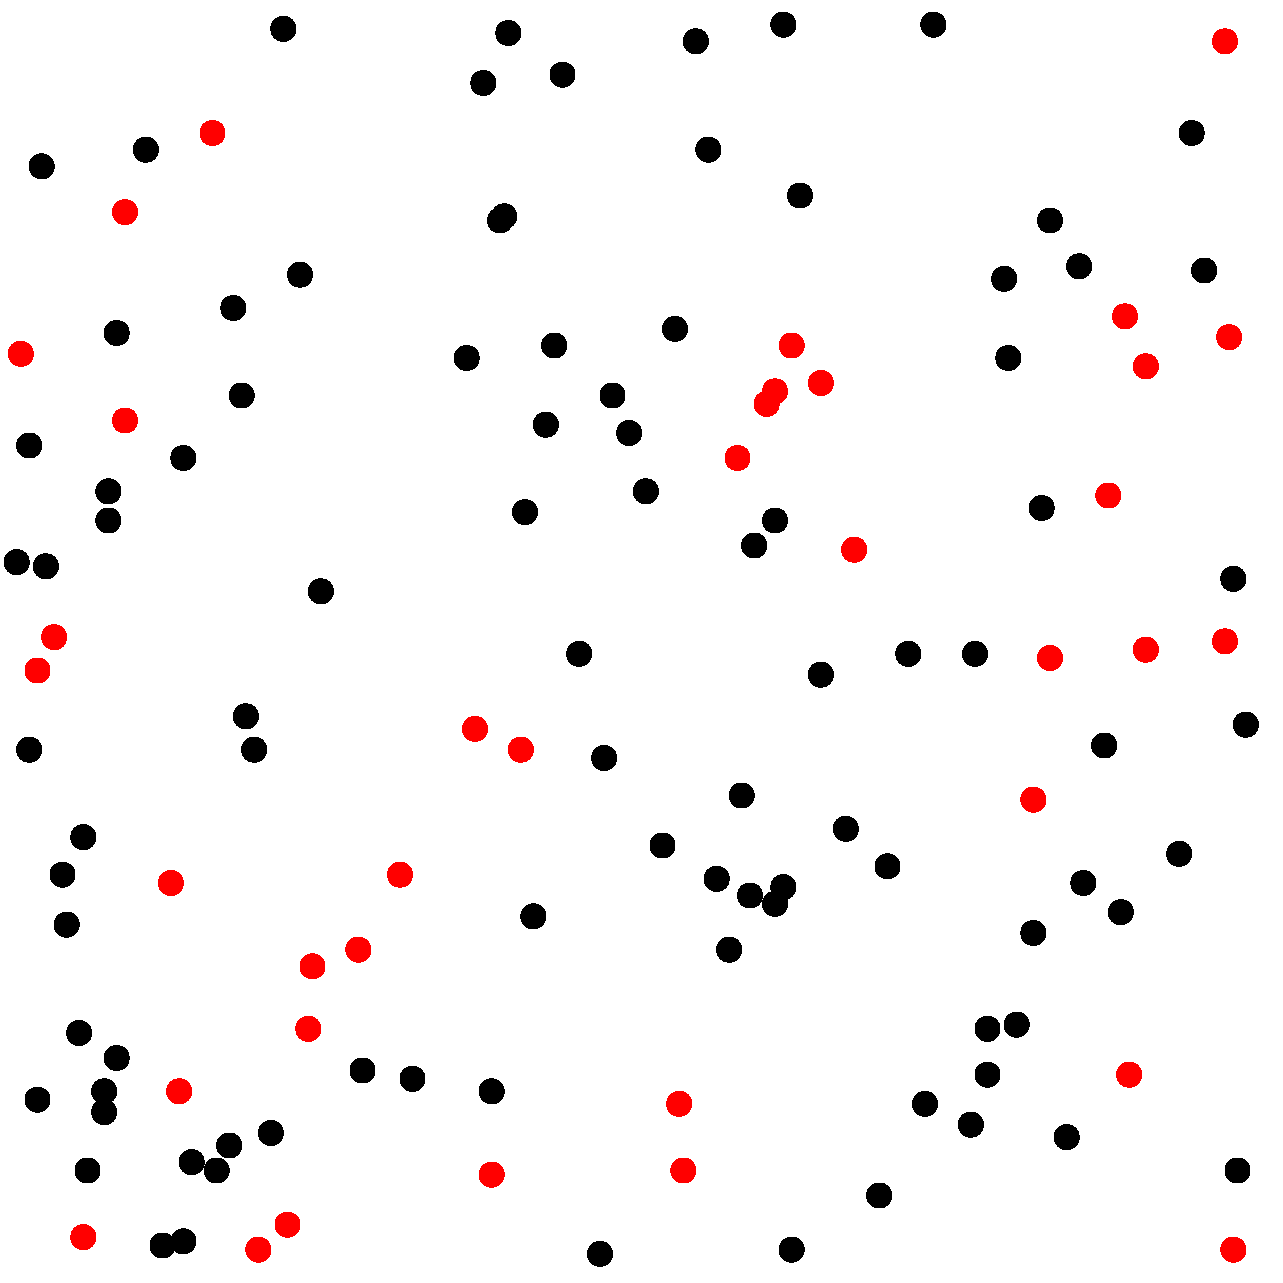
\includegraphics[width=4in]{red-black}}
\caption{Red-Black Point Process}
\label{fig:red-black-output}
\end{figure}

This particular algorithm can also be used through the existing
\texttt{Create\-RedBlack\-Propose}, and the \texttt{CreateFixedCheck} with
a probability of $1$.


% \emph{XXXX - should we put this section into this chapter rather than
%previous one?}

\section{Creating New Configuration Types}

For some problems, the supplied configuration types are not
sufficient.  Either the type of objects that make up the state are not
covered by the provided configuration types or the existing
configurations are not efficient enough.

As an example of the second case, if we had an algorithm that
performed a lot of checks to count the objects close to a particular
object, then it may be appropriate to use a different configuration
type that was more optimised for that sort of operation.  Such an
optimisation would be to sort the objects into bins according to where
they are located in the plane.  Now to find all objects within a given
radius $r$ of a particular object $y$, we only have to check the bins that
are within a radius $r$ of the bin that contains $y$.  While this
internal representation for the configuration speeds up these distance
checking operations, it slows down other operations such as counting
all objects in the configuration.

The creation of new configuration types requires knowledge of the
\GAP{} object model.  This is covered in the \emph{Programming in
\GAP{} 4} manual \cite{gap-prg} that is distributed with \GAP{}.

New configuration types must be derived from the abstract object
category \texttt{IsConfiguration}.  If a new object type is required,
it must derive from \texttt{IsPicture\-Object}.

Any new configuration must implement all the operations listed in the
previous section.  In addition to those operations, the new configuration
must implement a number of operations that are used to implement
various parts of GASP.  The extra operations are:
\begin{description}
\item[\texttt{AddObject}] - this operation is used to add an object to
the configuration.  It is not designed to be called by algorithms
directly.  Instead, it is used to implement change objects that add
objects to the configuration.  The prototype for this operation is:
\begin{lstlisting}{}
AddObject(config, object);
\end{lstlisting}
\item[\texttt{DelObject}] - this operation is used to delete an object
to the configuration.  As with \texttt{AddObject}, it is not designed
to be called by algorithms directly.  The prototype for this operation
is:
\begin{lstlisting}{}
DelObject(config, object);
\end{lstlisting}
\item[\texttt{DrawConfiguration}] - this operation is used to draw the
configuration of objects to a graphic sheet.  This will generally be
implemented by calling the \texttt{DrawObject} method on each object
in the configuration.  The prototype is:
\begin{lstlisting}{}
DrawConfiguration(config, graphicsheet);
\end{lstlisting}
\end{description}

The objects that make up the configuration need only implement a few
operations.  The two required operations are:
\begin{description}
\item[\texttt{SquareDistance}] - this operation calculates the square
of the distance between two objects.  The prototype for
\texttt{Square\-Distance} is:
\begin{lstlisting}{}
distance := SquareDistance(object, otherobject);
\end{lstlisting}
\item[\texttt{DrawObject}] - this operation is responsible for drawing
the object to an \XGAP{} graphic sheet.  The prototype for
\texttt{Draw\-Object} is:
\begin{lstlisting}{}
DrawObject(object, graphicsheet);
\end{lstlisting}
\end{description}

Provided that the new object type is implemented as an objectified
record, then the marks operations need not be implemented.  Otherwise,
those interfaces must be reimplemented for the object type.

For more information on implementing new configurations, see the
implementation of the \texttt{Point\-Configuration} type in the GASP
package.

\section{Change Objects}

Change objects are used in the GASP framework to represent all changes
made to configuration objects.  GASP comes with a number of useful
change object types, which were described in Section
\ref{sect:proposal-function-impl}.

New change objects must derive from the abstract category
\texttt{IsChange}.  A change object contains all the information that
is required to apply the change to the configuration, or to revert it
once applied.  These two actions on the configuration are handled by
the following two operations:

\begin{lstlisting}{}
ApplyChange(change, config);
RevertChange(change, config);
\end{lstlisting}

\noindent These operations must be implemented for each new change
type.  Usually a change object is implemented in terms of the
\texttt{AddObject} and \texttt{DelObject} operations of the
\texttt{Configuration} type, so that it may be used with more than one
configuration type.

It is also desirable that the new change object type implement the
standard \GAP{} operation \texttt{PrintObj}, which is used to print a
representation of the object to a file.  This operation will be called
when writing the type of change to the log file.  For this reason, it
is required that \texttt{PrintObj} write the code necessary to
recreate the object.  If this operation is not implemented correctly,
the usefulness of the log file is greatly reduced.

\subsection{The Log File}\label{sect:log-file}

Provided that the user turned on logging, all changes to the
configuration are written to a log file.  The lines in the log file
look similar to:

\begin{indent}
\texttt{[ }\emph{change}\texttt{, }\emph{acceptprob}\texttt{,
}\emph{accept}\texttt{ ]}
\end{indent}

\noindent Here, \emph{acceptprob} is the calculated probability of
accepting the change and \emph{accept} is a boolean representing
whether or not the change was actually accepted and applied.

The log file contains all the information required to replay the
simulation to recreate the final state of the simulation.  In fact, it
is possible to replay the simulation up to any point by using the
log.  This could be used to play back the simulation at a faster rate.

The log is also a useful source of statistics about the run of the
simulation.  For instance, we can look for patterns in the types of
changes that are proposed and the acceptance rates.  Some interesting
information the log could provide are:

\begin{itemize}
\item states for which proposals are given very low acceptance
probability.
\item lengths of runs of acceptances or rejections.
\item changes in the acceptance probability over time.
\end{itemize}

I have not completed the framework to used to parse the log file for
post simulation analysis.  When the log parsing framework is complete,
it will be added to the GASP package.  However, parsing the log is
very simple, as each line is a valid \GAP{} expression.  So it is
possible to read the log before the log parsing framework is complete.

% -*- mode: latex; mode: auto-fill -*-

\chapter{Conclusion}

The GASP package should prove to be a useful tool for simulation of
spatial statistical processes.  The package is designed to be as
extendable as possible, I expect that it will become more useful in
the future as more algorithms are added to the library accompanying
GASP.

In hindsight, it may have been a better decision to choose a different
language.  Parts of the framework that required floating point support
could only be tested by people who had access to the development
version of \GAP, as there are no publicly released versions of \GAP{}
with floating point support.  Once the next version of \GAP{} is
released, this barrier will be removed.

If GASP is too slow to run a simulation, \GAP{} comes with a \GAP{} to
C translator, which can increase the speed of a program.
Alternatively, GASP can be used to explore an algorithm, before using
another program to perform a longer simulation.

I plan to add some more features to GASP and submit it as a share
package for \GAP.


%% the bibliography
%\nocite{*}
\bibliography{thesis}
\bibliographystyle{plain}

\end{document}
